% !TEX program=pdflatex

\documentclass[x11names]{article}

\usepackage[style=authoryear]{biblatex}
\addbibresource{zugzwang.bib}

\usepackage{multirow}

% LNAI stuff

% TLP stuff

\usepackage{times}
% \usepackage{soul} % to strikeout, highline, etc.
\usepackage{url}
\usepackage[hidelinks]{hyperref}
\usepackage{graphicx}
\usepackage{booktabs}
\usepackage{algorithm}
\usepackage{algorithmic}
\urlstyle{same}
\usepackage[%textsize=tiny,
    prependcaption]{todonotes}
%

% OUR PACKAGES AND MACROS


\usepackage{tikz}
\tikzset{
    boxed/.style={draw, rectangle, rounded corners=4pt, fill=gray!10,inner sep=1em, anchor=center},
    event/.style={},
    smodel/.style={fill=gray!25},
    tchoice/.style={draw, circle},
    indep/.style={},
    proptc/.style = {-latex, dashed},
    propsm/.style = {-latex, thick},
    doubt/.style = {gray} }
\usetikzlibrary{calc, positioning, patterns, perspective}
%
\usepackage{hyperref}
\hypersetup{
    colorlinks=true,
    linkcolor=blue,
    citecolor=blue,
    urlcolor=blue, }
%
\usepackage{commath}
\newtheorem{assumption}{Assumption}
\usepackage{amssymb}
\usepackage[normalem]{ulem}
\usepackage[euler-digits,euler-hat-accent]{eulervm}
\usepackage[nice]{nicefrac}
\usepackage{stmaryrd}
\usepackage{acronym}
\usepackage{multicol}
\usepackage{multirow}
\usepackage{cleveref}
\crefname{example}{ex.}{exs.}
\crefname{proposition}{prop.}{props.}
\crefname{assumption}{asp.}{asps.}
\usepackage{hyphenat}
\hyphenation{
mo-dels mi-ti-ga-ted mi-ni-mal ex-am-ple spe-ci-fi-ca-tion
}

% Environments

\newtheorem{example}{Example}
\newtheorem{definition}{Definition}
\newtheorem{proposition}{Proposition}

% Commands

\def\tight{%
  \itemsep 0pt plus 1pt
  \parskip 0pt plus 1pt}

\newcommand{\ie}{\emph{i.e.}}
\newcommand{\eg}{\emph{e.g.}}
\newcommand{\eat}[1]{}
\newcommand{\at}[1]{\ensuremath{\!\del{#1}}}        %   argument
%
%   Notation
%
%   special sets
%
\newcommand{\cla}[1]{\ensuremath{{\cal #1}}}        %   class of something  
\newcommand{\clx}[1]{\ensuremath{{\mathbb{#1}}}}
%
%   connectives in logic programs
%
\newcommand{\conj}{\ensuremath{\wedge}} \newcommand{\disj}{\ensuremath{\vee}}
\newcommand{\clause}{\ensuremath{\leftarrow}}
\DeclareMathOperator{\naf}{\sim\!}
% \newcommand{\naf}{\ensuremath{\sim\!\!}}
\newcommand{\co}[1]{\ensuremath{\overline{#1}}}     %   complement
\renewcommand{\complement}{\ensuremath{\mathcal{C}}}     %   complement
%
%   often used sets
%
\newcommand{\ATOMSset}{\ensuremath{\cla{A}}}
\newcommand{\LITERALSset}{\ensuremath{\cla{L}}}
\newcommand{\PATOMset}{\ensuremath{\ATOMSset_{\cla{P}}}}
\newcommand{\FACTSset}{\ensuremath{\cla{F}}}
\newcommand{\PROBFset}{\ensuremath{\cla{P}}}
\newcommand{\RULESset}{\ensuremath{\cla{R}}}
\newcommand{\TCHOICEset}{\ensuremath{\cla{T}}}
\newcommand{\MODELset}{\ensuremath{\cla{M}}}
\newcommand{\EVENTSset}{\ensuremath{\cla{E}}}
\newcommand{\CONSISTset}{\ensuremath{\cla{W}}}
%
%   often used functions
%
%   error (loss)
\newcommand{\err}[1]{\ensuremath{\mathrm{err}\at{#1}}}
%
%   probability 
\newcommand{\prfunc}{\ensuremath{\mathrm{P}}}       
%   P(X = x)
\newcommand{\pr}[1]{\ensuremath{\prfunc\at{#1}}}    
%   P_X(x)
\newcommand{\prd}[1]{\ensuremath{\prfunc_{#1}}}     
\newcommand{\prT}{\prd{\TCHOICEset}}
\newcommand{\prM}{\prd{\MODELset}}
\newcommand{\prE}{\prd{\EVENTSset}}
\newcommand{\prC}{\prd{\cla{C}}}
%
%   local notation
%
 %   m(x)
\newcommand{\pw}[1]{\ensuremath{\mu\at{#1}}}           
%   m_T     total choices 
\newcommand{\pwT}{\ensuremath{\mu_{\TCHOICEset}}}   
%   m_T(x)
\newcommand{\pwt}[1]{\ensuremath{\pwT\at{#1}}}     
%   m_M     stable models  
\newcommand{\pwM}{\ensuremath{\mu_{\MODELset}}}   
%   m_M(x)
\newcommand{\pwm}[1]{\ensuremath{\pwM\at{#1}}}     
%   m_C     eq. classes 
\newcommand{\pwC}{\ensuremath{\mu_{\textrm{\cla{C}}}}}   
%   m_C(x)
\newcommand{\pwc}[1]{\ensuremath{\pwC\at{#1}}}     
%   m_E     events 
\newcommand{\pwE}{\ensuremath{\mu_{\EVENTSset}}}   
%   m_E(x)
\newcommand{\pwe}[1]{\ensuremath{\pwE\at{#1}}}     
%
%
%
\newcommand{\stablecore}[1]{\ensuremath{\left\llbracket #1 \right\rrbracket}}
\newcommand{\inconsistent}{\bot}
\newcommand{\given}{\ensuremath{~\middle|~}}
\newcommand{\consequenceclass}{\ensuremath{\Lambda}}
\newcommand{\indepclass}{\ensuremath{\Diamond}}
\newcommand{\probfact}[2]{\ensuremath{#1:#2}}
\newcommand{\probrule}[3]{\probfact{#1}{#2} \leftarrow #3}
\newcommand{\class}[1]{\ensuremath{[{#1}]_{\sim}}}
\newcommand{\tcgen}[1]{\MODELset\at{#1}}
\newcommand{\condsymb}[2]{\ensuremath{p_{#1|#2}}}
\newcommand{\lpmln}{\texttt{LP\textsuperscript{MLN}}}
\newcommand{\emptyevent}{\ensuremath{\lambda}}
\newcommand{\powerset}[1]{\ensuremath{\mathbb{P}\at{#1}}}
%
%   Acronyms
%
\acrodef{BK}[BK]{background knowledge}
\acrodef{ASP}[ASP]{answer set program}
\acrodef{NP}[NP]{normal program}
\acrodef{LP}[LP]{logic program}
\acrodef{PCR}[PCR]{program with choice rules}
\acrodef{DS}[DS]{distribution semantics}
\acrodef{PF}[PF]{probabilistic fact}
\acrodef{TC}[TC]{total choice}
\acrodef{SM}[SM]{stable model}
\acrodef{SC}[SC]{stable core}
\acrodef{KL}[KL]{Kullback-Leibler}
\acrodef{SBF}[SBF]{simple but fruitful}
\acrodef{RSL}[RSL]{random set of literals}
\acrodef{RCE}[RCE]{random consistent event}
\acrodef{SASP}[SASP]{stochastic answer set program}
\acrodef{WASP}[WASP]{weighted answer set program}
\acrodef{HMM}[HMM]{hidden Markov model}
%
%   Common objects
%
\newcommand{\sbf}{\ensuremath{\mathrm{sbf}}}
%
%   Reviewing
%
\newcounter{revcounter}
\newcommand{\LOOK}{\ensuremath{\blacksquare}}
\newcommand{\delete}[1]{\sout{#1}}
\newcommand{\sidenote}[1]{\stepcounter{revcounter}{\color{red!50!black}\(\vert^{\arabic{revcounter}}\)}\marginpar{{\color{red!50!black}\(^{\arabic{revcounter}}\vert\)}\footnotesize #1}}
\newcommand{\replace}[2]{\delete{#1}\sidenote{#2}}
%\newcommand{\franc}[1]{{\color{green!30!black}#1}}
\newcommand{\bruno}{\color{red!60!black}}
%\newcommand{\spa}[1]{{\color{brown!80!black}{#1}}}
\newcommand{\dietmar}[1]{{\color{brown!40!black}#1}}

% -- side notes --

\newcommand{\selfnote}[1]{\todo[backgroundcolor=green!20]{{\footnotesize #1}}}
\newcommand{\spa}[1]{{\todo[size=footnotesize,color=teal!20]{\textbf{SPA:} #1}}}
\newcommand{\dsnote}[1]{{\todo[size=footnotesize,color=teal!20]{\textbf{DS:} #1}}}
\newcommand{\franc}[1]{{\todo[size=footnotesize,color=green!30]{\textbf{FC:} #1}}}
\newcommand{\bdnote}[1]{{\todo[size=footnotesize,color=red!60]{\textbf{BD:} #1}}}

\usepackage{geometry}
\geometry{
    paper=a4paper,
    left=1cm,
    right=5cm,
    top=1cm,
    bottom=2cm
}

\title{Weighted Answer Set Programs}
\author{Francisco, Bruno, Salvador, Dietmar}

\begin{document}

\maketitle

\begin{abstract}
    Drawing inspiration from HMMs; State of the art of PLP and Probabilistic ASP; Leveraging current Prob ASP systems; 
\end{abstract}

Using a \acl{LP} to model and reason over a real world situation is often complicated because of uncertainty underlying the problem being worked on.
Classic \aclp{LP} represent knowledge in precise terms, which turn out to be problematic when the application data is affected by stochastic factors, which is frequently the case.

\section{Uncertainty and ASPs}


\begin{figure}[t]
	\begin{center}
		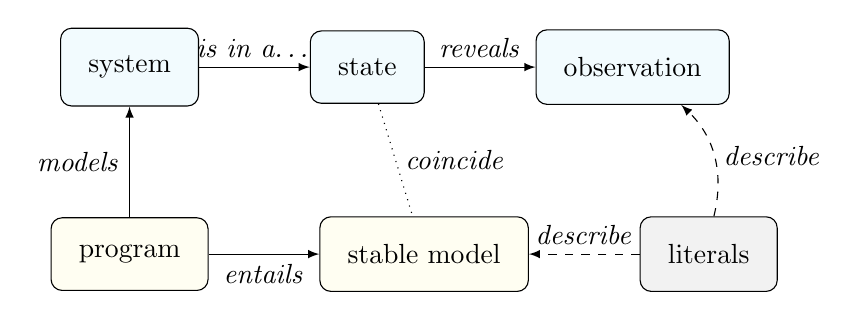
\begin{tikzpicture}[node distance=4em]
            \node[boxed, fill=cyan!5] (A) {system};
			\node[boxed, right = of A, fill=cyan!5] (S) {state};
			\node[boxed, right = of S, fill=cyan!5] (z) {observation};
			\node[boxed, below = of A, fill=yellow!5] (P) {program};
			\node[boxed, right = of P, fill=yellow!5] (m) {stable model};
			\node[boxed, right = of m] (L) {literals};
			% ----
            \path[-latex] 
                (A) edge node[above] {\emph{is in a\ldots}} (S)
                (P) edge node[left] {\emph{models}} (A)
                (S) edge node[above] {\emph{reveals}} (z)
                (S) edge[dotted,-] node[right] {\emph{coincide}} (m)
                (L) edge[bend right, dashed] node[right] {\emph{describe}} (z)
                (L) edge[dashed] node[above]{\emph{describe}} (m)
                (P) edge node[below] {\emph{entails}} (m);
		\end{tikzpicture}
	\end{center}

	\caption{%
		}
\end{figure}

\Acp{HMM} setup a well known, widely used, framework to describe and study partially observable stochastic processes\sidenote{HMMs stress the \textbf{process} and we are not looking into that.}. Briefly, a \ac{HMM} process is described by a sequence of states, each defined as a set of random variables that are partially observed. This means that (1) observation of states include only a fixed subset of those variables, and also that (2) the observed values are subject to random perturbations.

We try to capture both the partial observability and the stochastic nature of a system in a logic setting. To this end we think of a system, $S$, as a formal model, $P$, together with a set of observations, $D$:

\begin{equation}\label{eq:def.system}
    S = \left( P, D \right)
\end{equation}

The formal model is an \acl{ASP} extended with \emph{weights}, that we describe later in this paper, and such that the \aclp{SM} of the program are the system states. On the other hand, any given system state can be (or has been) observed. The outcome of each single observation is a set of literals of that program.

\begin{example}[Coins, Dices, and Cards]
    Consider a scenario where a coin is tossed and, if the result is \emph{heads}, \(a\), then a dice is thrown, \(b\), or a card is drawn, \(c\). If the coin lands in \emph{tails}, \(\neg a\), no information is given. A formal model of this system is the program  
    \begin{equation}\label{eq:derived.fruitful}
        P_{\sbf} = \left\lbrace\begin{aligned}
            a \vee \neg{a}  & ,          %
            \\
            b \vee c        & \clause a
        \end{aligned}
        \right.
    \end{equation}
    that has atoms \(\set{a, b, c}\), literals \(\set{a, \neg a, b, \neg b, c, \neg c}\) and \aclp{SM}
    \begin{equation}
        \set{a, b}, \set{a, c}, \set{\neg a}.
    \end{equation}
    
    Possible observations include:
    \begin{itemize}
        \item \(\set{a,c}\): a \ac{SM}, therefore a system state, observed \emph{heads} and \emph{card}.
        \item \(\set{a}\): not a \ac{SM} but contained in the two \acp{SM} $\set{a, b}$ and $\set{a, c}$, observed \emph{heads} but we have no information about the \emph{cards} or the \emph{dice}.
        \item \(\set{\neg a, \neg b}\): not a \ac{SM} but contains the \ac{SM} $\set{\neg a}$, the coin was observed as \emph{not heads} (\emph{tails}?); also we are certain that no card was drawn but have no information about the dice.
        \item \(\set{b,c}\): not related with any \ac{SM}.
        \item \(\set{a,\neg a}\): an inconsistent observation.
    \end{itemize}    
\end{example}

We use sets of literals, instead of atoms, to represent observations because they make possible the distintion between a \emph{explicit negative observation} \(\neg\alpha\) (\eg ``I see tails.'') and \emph{not observed} \(\naf \alpha\) (\eg ``The coin in hidden.''). This corresponds to assuming a ``boolean sensor'' for each $\alpha$ and $\neg \alpha$.

So, the program \ref{eq:derived.fruitful} defines the ``sensors''
\begin{equation*}
    a, \neg a, b, \neg b, c, \neg c
\end{equation*}

\nocite{*}

\printbibliography
\end{document}